\documentclass[10pt,a4paper]{article}
\usepackage[utf8]{inputenc}
\usepackage[T1]{fontenc}
\usepackage{lmodern}
\usepackage[margin=1.5cm, top=1.4cm, bottom=1.4cm]{geometry}
\usepackage{hyperref}
\usepackage{enumitem}
\usepackage{titlesec}
\usepackage{xcolor}
\usepackage{graphicx}

\definecolor{accent}{HTML}{00686E}
\hypersetup{colorlinks=true, urlcolor=accent, linkcolor=accent}
\pagenumbering{arabic}
\setlength{\parindent}{0pt}

\titleformat{\section}{\large\bfseries\color{accent}}{}{0em}{}[\vspace{-0.6em}\rule{\textwidth}{0.8pt}]
\titlespacing{\section}{0pt}{7pt}{4pt}

\newcommand{\role}[4]{%
  \textbf{#1} \hfill \textbf{#2}\\[1pt]%
  \textit{#3} \hfill \textit{#4}\\[2pt]%
}
\setlist[itemize]{leftmargin=1.2em, itemsep=1.5pt, topsep=2pt, parsep=0pt}

\begin{document}

% ================= HEADER =================
\begin{minipage}[c]{0.80\textwidth}
  {\Huge\bfseries Prabhavit Gupta}\\[3pt]
  {\color{accent}\large AI Engineer: LLM Workflows, TypeScript Architectures \& Agentic Systems}\\[6pt]
  {\footnotesize +39 351 610 7807 ~$\vert$~
  \href{mailto:prabhavitg@gmail.com}{prabhavitg@gmail.com} ~$\vert$~
  \href{https://www.linkedin.com/in/prabhavit/}{linkedin.com/in/prabhavit} ~$\vert$~
  \href{https://github.com/prab-gupta}{github.com/prab-gupta} ~$\vert$~
  Venice, Italy (EU Permanent / Milan On-Site Ready)}
\end{minipage}\hfill
\begin{minipage}[c]{0.18\textwidth}
  \raggedleft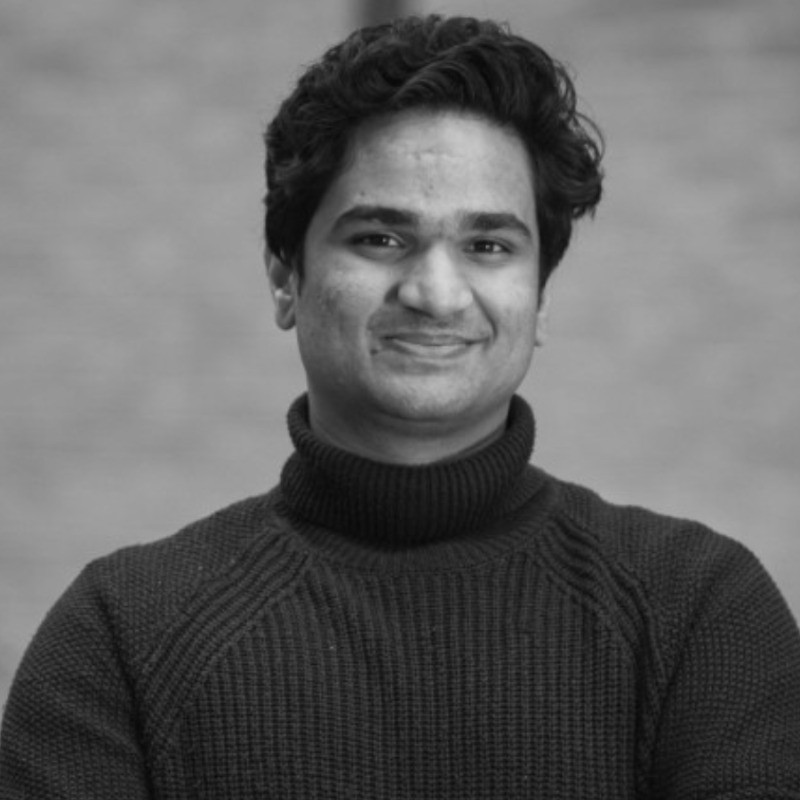
\includegraphics[width=2.0cm]{photo.jpg}
\end{minipage}
\vspace{-2pt}

% ================= SUMMARY =================
\section{Summary}
AI Engineer and Lead Developer with 3 years of hands-on production experience designing, building, and deploying reliable LLM-driven workflows, agentic tool orchestration, and data extraction pipelines. Proven track record turning raw unstructured document inputs into high-fidelity structured outputs, integrating vector retrieval/RAG, and architecting robust TypeScript/Node.js backend pipelines with PostgreSQL. Deep experience establishing rigorous evaluation frameworks, tracing real user transcripts, and tuning prompt schemas to maximize accuracy, eliminate hallucinations, and reduce latency. Native user of Claude Code, Codex, and agent swarms to ship production software rapidly. Holder of an EU Long-Term Residence Permit (permanent unrestricted EU work authorization across all EU member states, no sponsorship required); based in Venice, Italy and immediately available for on-site work and relocation to Milan.

% ================= TECHNICAL EXPERTISE =================
\section{Technical Expertise}
\begin{itemize}
  \item \textbf{LLM \& Agentic Engineering:} LLM APIs (OpenAI, Anthropic), agent tool orchestration, structured JSON outputs, RAG and semantic search, embeddings, vector databases, prompt engineering, context optimization, transcript-driven evaluation harnesses.
  \item \textbf{Backend \& TypeScript Development:} TypeScript, JavaScript, Node.js, Next.js, RESTful API design, PostgreSQL schema modeling, asynchronous job queues, Docker containerization.
  \item \textbf{Reliability \& Observability:} Error recovery, retry policies, schema validation, telemetry and trace monitoring (Sentry, PostHog), automated regression testing with Playwright.
  \item \textbf{Workflow Automation \& Integration:} n8n, webhook consumers, third-party API synchronization, data normalization, automated document extraction pipelines.
  \item \textbf{AI Tooling \& Workflow:} Claude Code, OpenAI Codex, cursor-based AI development, git, CI/CD pipelines.
  \item \textbf{Languages \& Work Authorization:} English (C1 Professional, fluent), Hindi (Native), Italian (Beginner). EU Long-Term Residence Permit (unrestricted EU work authorization across all EU member states, no sponsorship required).
\end{itemize}

% ================= EXPERIENCE =================
\section{Experience}

\role{\href{https://flowspace.co}{FlowSpace.co}}{Mar 2024 - Aug 2026}{Lead Developer \& AI Systems Architect}{London, UK (remote)}
\begin{itemize}
  \item Built and operated production customer-facing AI agents on a marketplace platform serving 4,500+ active users, handling complex inquiries against live platform data and APIs.
  \item Developed automated document and web data parsing pipelines with LLM extraction, converting unstructured partner data into validated JSON schemas and expanding live platform inventory.
  \item Engineered human-in-the-loop escalation workflows and multi-step reasoning chains with strict tool constraints, ensuring zero ungrounded responses in customer-facing flows.
  \item Iterated system prompts and tool schemas against real production transcripts, systematically lowering edge-case error rates and measuring response quality against ground-truth datasets.
  \item Maintained resilient backend integrations with TypeScript/Node.js and PostgreSQL, implementing asynchronous queues and automated retries for high-throughput reliability.
  \item Built automated end-to-end integration and regression test suites with Playwright, ensuring API contract validity and zero regressions across continuous release cycles.
\end{itemize}

\role{Urlink}{Apr 2025 - Jul 2025}{Project Manager \& Solutions Developer (Freelance)}{Barcelona, Spain (remote)}
\begin{itemize}
  \item Led technical discovery and implementation of customized web solutions and automated data processing pipelines for client platforms.
  \item Built automated data ingestion and transformation services connecting third-party APIs to PostgreSQL datastores, maintaining high data freshness and integrity.
  \item Delivered interactive functional prototypes to validate user flows and technical requirements prior to sprint execution, accelerating cycle times.
\end{itemize}

\role{Independent Technical Consultant}{Aug 2023 - Feb 2024}{AI Automation \& Integration Developer}{Venice, Italy}
\begin{itemize}
  \item Designed, deployed, and supported tailored LLM integrations, document-parsing pipelines, and webhook orchestration workflows for European clients using TypeScript, Python, and n8n.
  \item Replaced fragile manual data entry workflows with automated sync pipelines featuring structured error handling, retry policies, and alerting.
  \item Documented system architectures and delivered technical walkthroughs, ensuring smooth client adoption and high operational reliability.
\end{itemize}

% ================= EDUCATION =================
\section{Education}
\role{Ca' Foscari University of Venice}{2020 - 2024}{BA in Philosophy, International Studies and Economics}{Venice, Italy}
\begin{itemize}
  \item Rigorous training in formal logic, analytical problem solving, systems analysis, and macroeconomic decision models.
\end{itemize}

\end{document}
